\section{Process Definition}

\subsection{Emergency Services Crew}
\begin{enumerate}

    \item \textbf{Receive and Assess Call.} 
    The \textit{Emergency Call Agent} receives incoming calls and collects relevant details about the incident. 
    This task requires human input for accurate interpretation and contextual understanding of the caller's description, 
    ensuring critical information is gathered effectively. The information that this agent receives answers the following 
    six questions and is saved in a report:
    \begin{itemize}
        \item What type of fire is it? E.g. ordinary, electrical, gas, etc.
        \item Where is it? The location is received as coordinates \((x, y)\).
        \item Is anyone injured? How badly? The answer will be a list of strings, detailing the risk level of each person. If the list 
        if empty then there will be no injured people and it will be unnecessary to report it to the \textit{Medical Service Crew.}
        \item How severe is the fire? It will be considered as low, medium or high.
        \item Are there hazards? Examples of hazards could include gas cylinders, chemicals, explosions, etc.
        \item Is it an indoor or outdoor fire? The answer will be either \textit{outdoor} or \textit{indoor}.
        \item Is anyone inside or trapped? The answer will be an integer number $M$ representing the number of trapped people. 
        If $M > 0$, rescues are needed, and the \textit{Notification Agent} will detail that to the Fire Fighters Crew.
    \end{itemize}
    

    \item \textbf{Notify Other Crews Decision.} 
    The \textit{Notification Agent} receives the details about the fire then it decides which crew should be notify and send
    all the information to the flow. It also decides whether the medical services are required or not, depending on the 
    human input related to the injured individuals.    

\end{enumerate}

\paragraph{Task Dependencies:}

The sequential workflow for the Emergency Services Crew depends on task dependencies to ensure efficiency and coordination:
\begin{itemize}
    \item The \textit{Notify Other Crews Task} depends on the completion of the \textit{Receive and Assess Call Task}, which 
    involves human input to accurately assess and interpret the situation.
\end{itemize}


The task dependencies and agents who perform each task can be observed in Figure~\ref{fig:emergency_services_flow}.

\begin{figure}[h!]
	\centering
	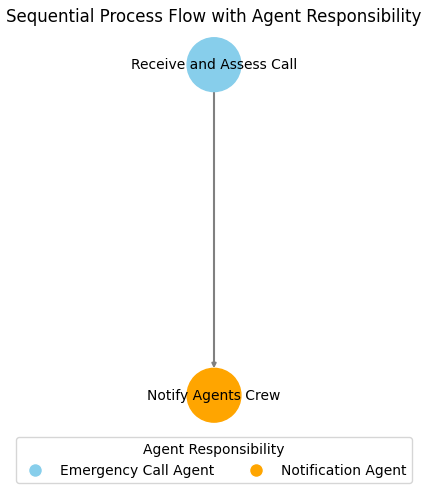
\includegraphics[height=0.4\textheight]{figures/emergency_services_crew_flow.png}
	\caption{Sequential Process Flow of the Medical Services Crew with Agent Responsibilities}
	\label{fig:emergency_services_flow}
\end{figure}

\subsection{Firefighter Agent Crew}

The Firefighter Agent Crew operates within a structured \textbf{sequential process} to ensure effective and coordinated response to fire emergencies. Each task is assigned to a specific agent with well-defined responsibilities, as detailed below:

\begin{enumerate}
    \item \textbf{Receive Report:} The \textit{Fire Chief} receives a fire assessment from the Emergency Service Operator. This serves as the starting point of the process, containing critical information such as the location and severity of the fire.
    \item \textbf{Allocate Firefighting Resources:} The \textit{Equipment Technician} determines if there exact resources required to combat the fire in question.
	\item \textbf{Deploy Fire Combatants:} The \textit{Fire Combatants} are deployed to the place of the fire, reporting an estimation of the time of arrival and a list of the fire fighting activities that will have to be performed.
	\item \textbf{Report Firefighting Response:} The \textit{Fire Chief} reports back a comprehensive summary of the firefighting activities.
\end{enumerate}

\paragraph{Task Dependencies}
The sequential process relies on strict task dependencies to maintain an organized workflow:
\begin{itemize}
    \item \textit{Allocate Firefighting Resources} depends on the completion of \textit{Receive Report}.
    \item \textit{Deploy Fire Combatants} depends on the completion of \textit{Deploy Fire Combatants}.
    \item \textit{Report Firefighting Response} depends on the completion of \textit{Deploy Fire Combatants}.
\end{itemize}

The visual representation in Figure~\ref{fig:firefighter_flow} highlights these dependencies and assigns colors to denote the responsible agents.

\begin{figure}[ht!]
	\centering
	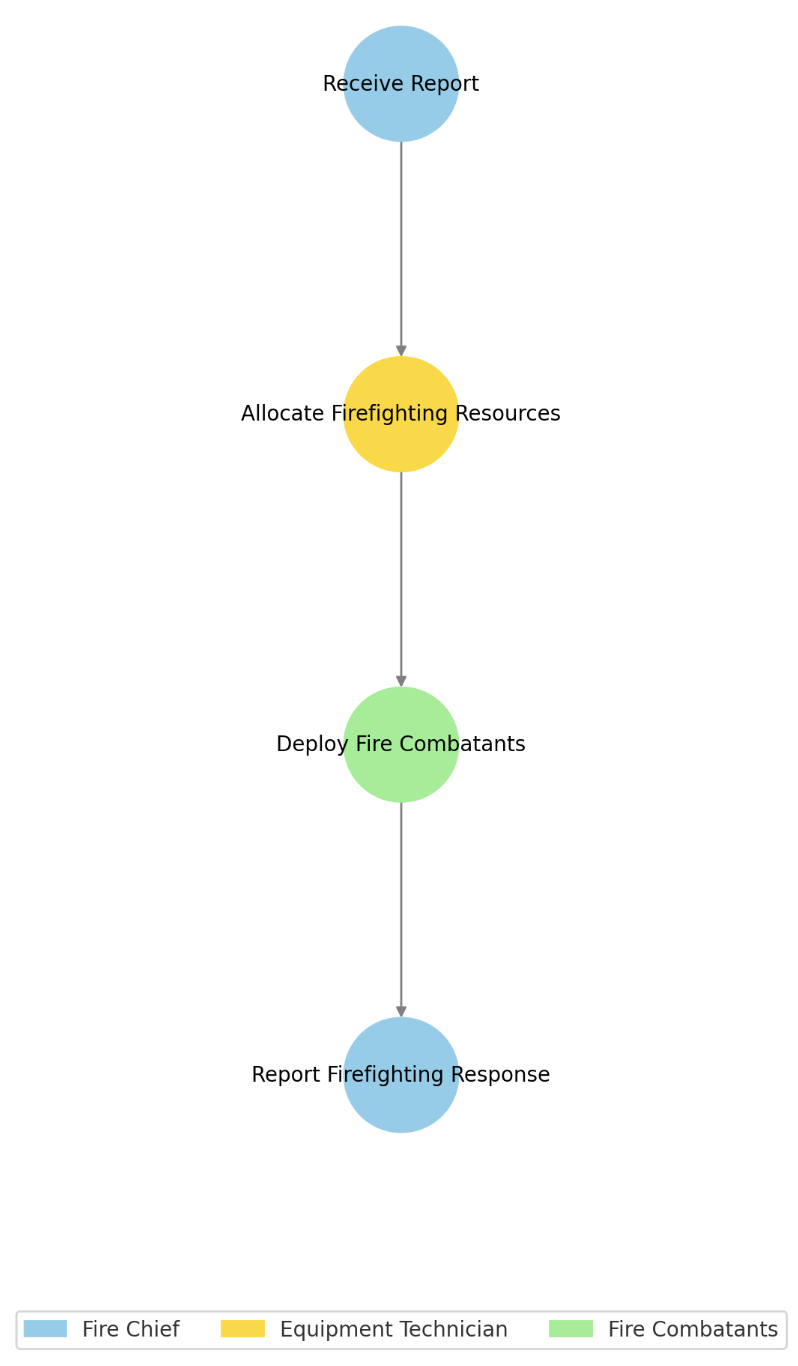
\includegraphics[height=0.59\textheight]{figures/Firefighter_Crew_Flow.png}
	\caption{Sequential Process Flow of the Firefighter Crew with Agent Responsibilities}
	\label{fig:firefighter_flow}
\end{figure}

\subsection{Medical Services Crew}

The Medical Services Crew operates follows a \textbf{sequential} task structure to plan the treatment and evacuation of injured people from the emergency site. The tasks included within the Medical Services are:

\begin{enumerate}
	\item \textbf{Receive Report:} The \textit{Medical Services Operator} receives the medical assessment of the fire incident, and parses key information, such as the location, the number of injured, and the severity of injuries.
	
	\item \textbf{Rank Hospitals:} The \textit{Hospital Coordinator} ranks the city's hospitals based on distance to the emergency location.

	\item \textbf{Allocate Hospital Resources:} The \textit{Hospital Coordinator} assesses the available resources (beds, ambulances, paramedics) at the hospitals, and allocates their resources according to the needs of the emergency.
	
	\item \textbf{Deploy Paramedics:} The \textit{Paramedics} plan their deployment to the place of the incident, reporting the total number of paramedics and ambulances dispatched, as well as their estimated times of arrival, and any special equipment that they could need.
	
	\item \textbf{Report Medical Response:} The \textit{Medical Services Operator} reports back a comprehensive summary of the response plan.
\end{enumerate}

\paragraph{Task Dependencies}
The sequential nature of the process requires to establish task dependencies to define the crew's workflow:
\begin{itemize}
	\item The \textit{Rank Hospitals} task depends on the completion of the \textit{Recieve Report} task.
	\item The \textit{Allocate Hospital Resources} task depends on the completion of \textit{Rank Hospitals}.
	\item The \textit{Deploy Paramedics} task depends on the completion of \textit{Allocate Hospital Resources}.
	\item The \textit{Report Medical Response} task depends on the completion of \textit{Deploy Paramedics}.
\end{itemize}

The task dependencies and agents who perform each task can be observed in Figure~\ref{fig:medical_services_flow}.

\begin{figure}[ht!]
	\centering
	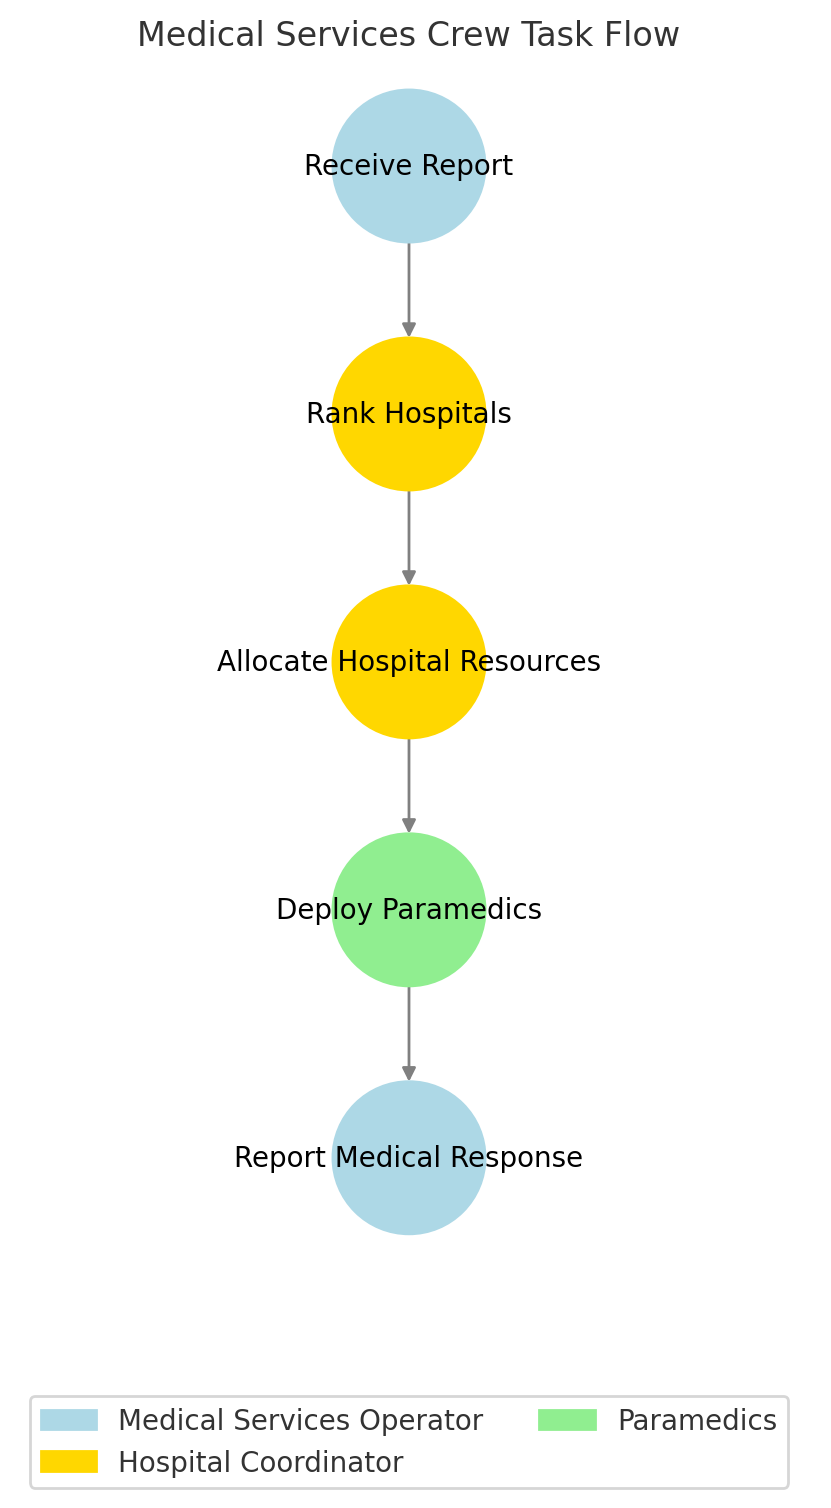
\includegraphics[height=0.6\textheight]{figures/Medical_Services_Crew_Flow.png}
	\caption{Sequential Process Flow of the Medical Services Crew with Agent Responsibilities}
	\label{fig:medical_services_flow}
\end{figure}

\subsection{Public Communication Crew}

The Public Communication Crew operates within a structured \textbf{sequential process} to ensure efficient and accurate communication of fire incident reports to the public. Each task is assigned to a specific agent with well-defined responsibilities, as detailed below:

\begin{enumerate}
	\item \textbf{Receive Report:} The \textit{Communication Operator} obtains the call assessment, fire report, and medical report in Markdown format. This serves as the starting point for the process and can filter any information that is not relevant for this crew.
	\item \textbf{Search Related Cases:} The \textit{Archive Keeper} searches for past incidents with similar locations or fire types. This task depends on the completion of the \textit{Receive Report} task.
	\item \textbf{Draft Initial Article:} The \textit{Article Writer} drafts an initial article based on the current report. This task also depends on the completion of the \textit{Receive Report} task.
	\item \textbf{Integrate Additional Information:} The \textit{Article Writer} integrates insights from related cases into the draft. This task requires the completion of both the \textit{Search Related Cases} and \textit{Draft Initial Article} tasks.
	\item \textbf{Review and Authorize Publication:} The \textit{Mayor} reviews the article and either authorizes publication or provides feedback for revisions. This task depends on the completion of the \textit{Integrate Additional Information} task.
	\item \textbf{Provide Social Media Feedback:} The \textit{Social Media Commentator} critiques the emergency response in a humorous yet constructive manner. This task depends on the approval of the article by the \textit{Mayor}.
\end{enumerate}

\begin{figure}[ht!]
	\centering
	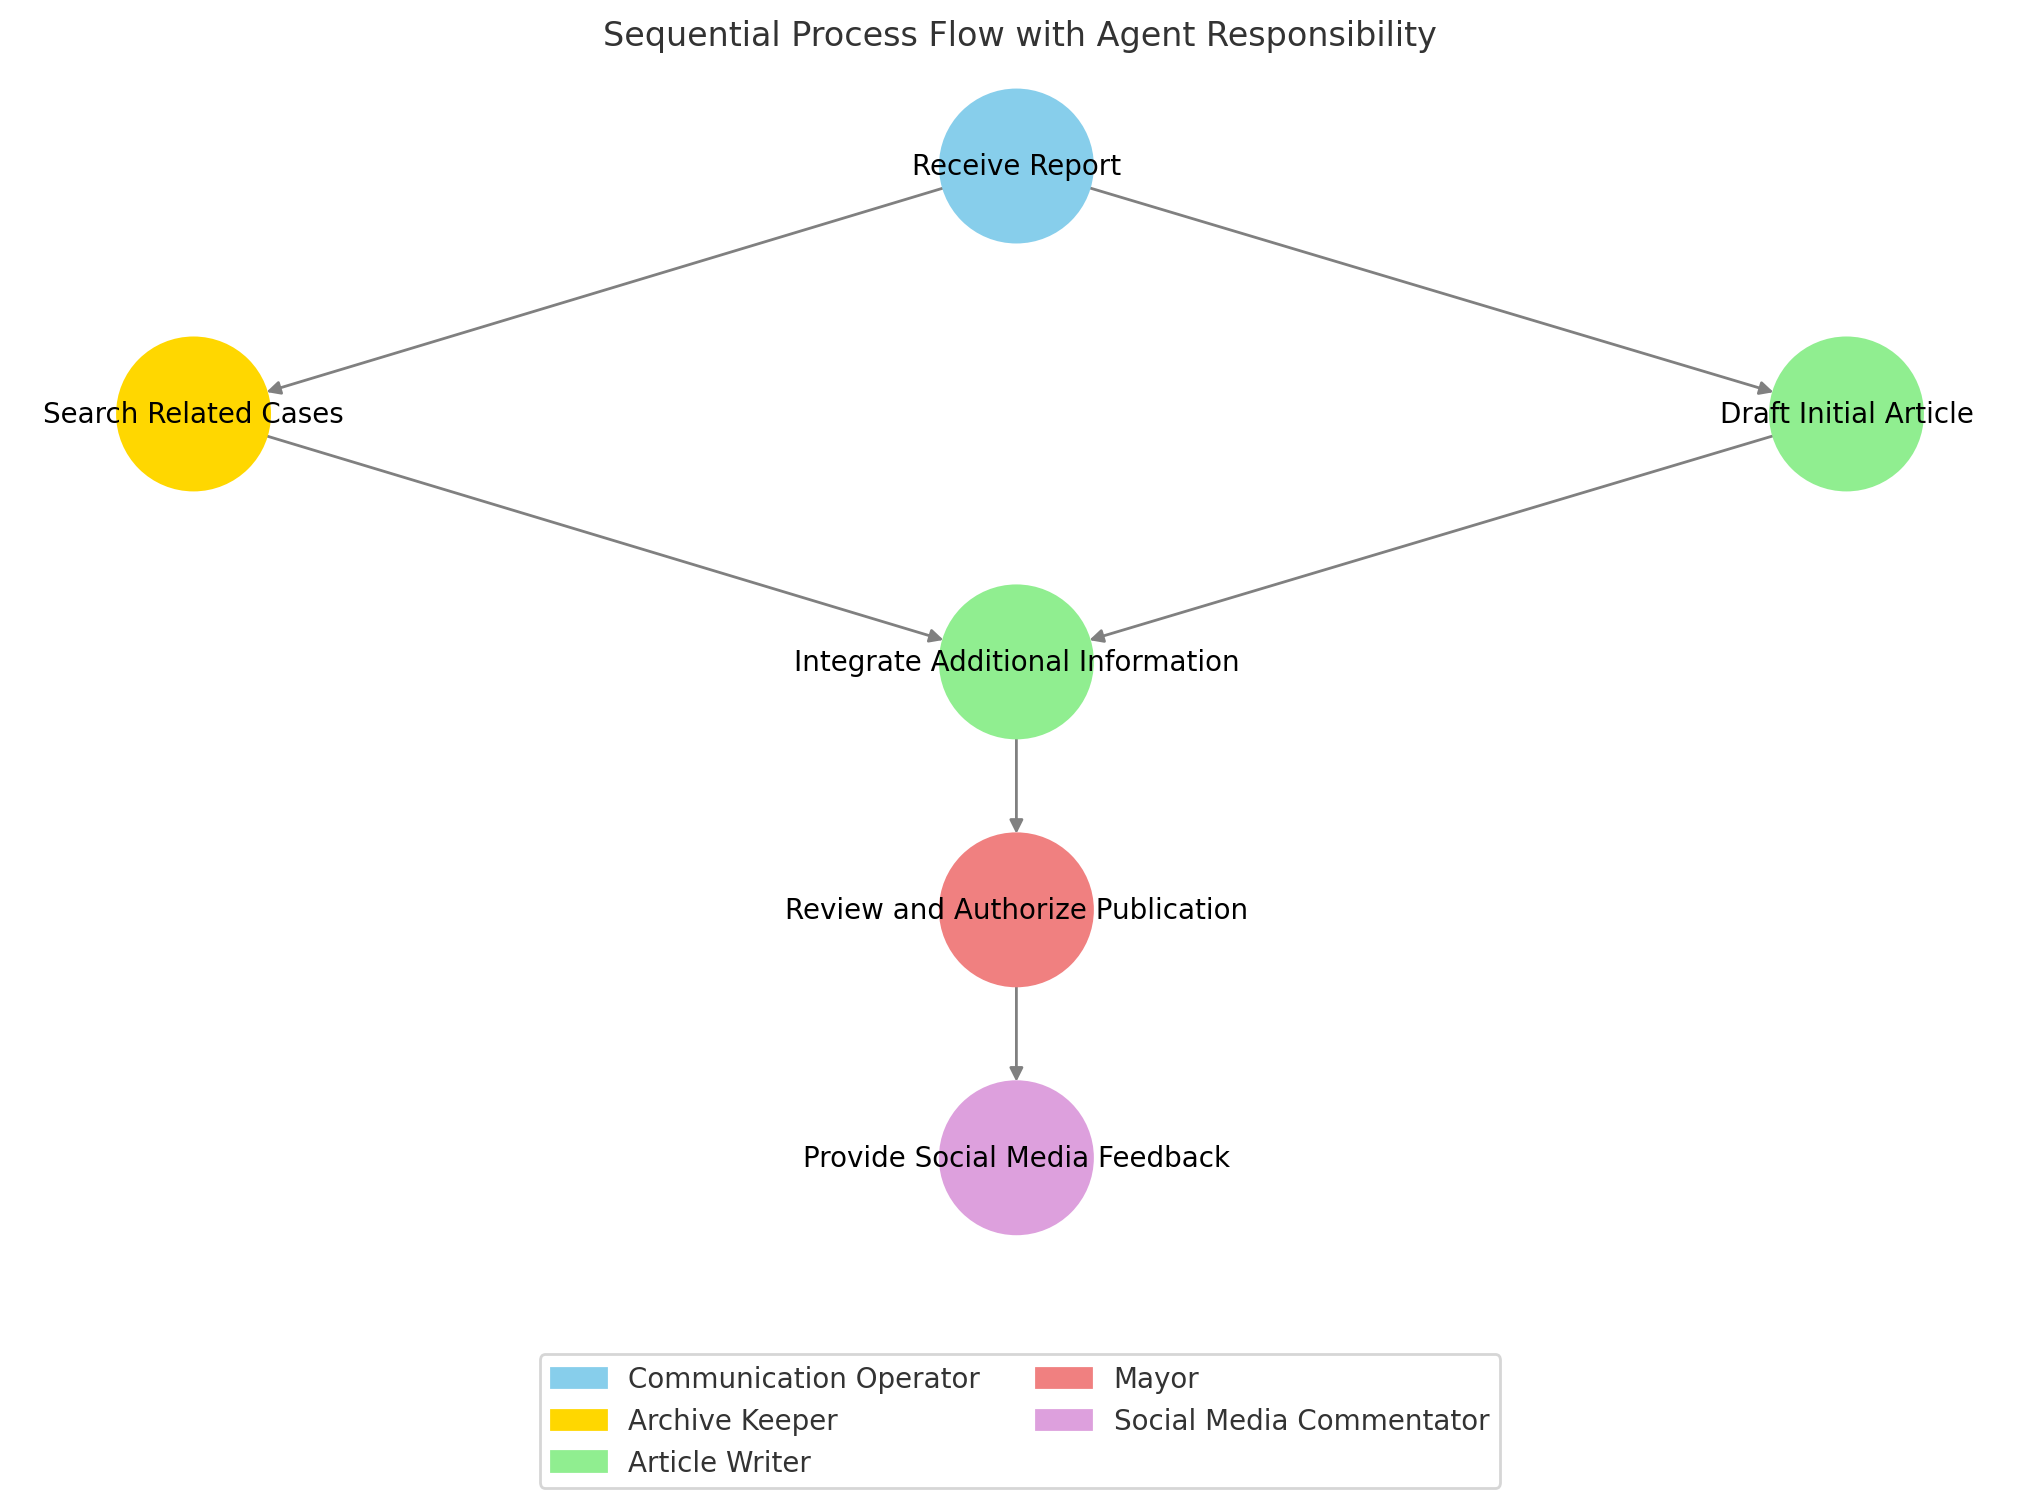
\includegraphics[width=0.4\textwidth]{figures/PC-process.png}
	\caption{Sequential Process Flow of the Public Communication Crew with Agent Responsibilities}
	\label{fig:public_comm_flow}
\end{figure}


\paragraph{Task Dependencies}
The sequential process relies on strict task dependencies to ensure an organized workflow:
\begin{itemize}
	\item \textit{Search Related Cases} and \textit{Draft Initial Article} can be executed in parallel but both depend on \textit{Receive Report}.
	\item \textit{Integrate Additional Information} requires the completion of both \textit{Search Related Cases} and \textit{Draft Initial Article}.
	\item \textit{Review and Authorize Publication} depends on \textit{Integrate Additional Information}.
	\item \textit{Provide Social Media Feedback} requires article approval from the \textit{Mayor}.
\end{itemize}

The visual representation in Figure~\ref{fig:public_comm_flow} highlights these dependencies and assigns colors to denote the responsible agents, ensuring clarity and accountability.
